\documentclass[a4j]{jarticle}
\renewcommand{\baselinestretch}{0.9}
\setlength{\textwidth}{16.92cm}
\setlength{\textheight}{24.6cm}
\setlength{\oddsidemargin}{-0.50 cm}
\setlength{\evensidemargin}{-0.50 cm}
%\setlength{\oddsidemargin}{0 cm}
\setlength{\topmargin}{-1.5cm}%{-0.8 cm}
\setlength{\abovedisplayskip}{-2.0cm}
\setlength{\belowdisplayskip}{-2.0cm}
\usepackage[dvipdfmx]{graphicx}

\begin{document}
%
\begin{center}
  {\Large \underline{特別研究報告審査会に関するアンケート}}
\end{center}
\begin{flushright}
  {\normalsize システム最適化研究室 大原源悠}
\end{flushright}
%

いつもお世話になっております。システム最適化研究室の大原源悠と申します。今回は、特別研究報告審査会についてのアンケートにご協力いただきたくご連絡させて頂きました。\\

私は、「特別研究報告審査会のより柔軟なスケジュールの作成」を特別研究のテーマとし、研究を行っています。現在、ある先生から、特別研究報告審査会のスケジュール作成について、追加したい要件があるという要望を頂いております。このことから、スケジュール作成において、ほかにも追加・変更したい部分があるかどうかの調査を行うためにこのようなアンケートを実施いたしました。\\

まず、現在のスケジュール作成問題について説明いたします。\\
現在のスケジュールは、スケジュールが満たすべき要件を、絶対制約と考慮制約の$2$つに分け、スケジュール
を作成しています。絶対制約とは、「学生は、自分自身と単教員がともに参加可能なセッションで発表する」や、「研究室が同じ学生は教室をまたいで同時刻のセッションで発表しない」などの必ず満たさなければならない制約のことです。考慮制約とは、「同時刻に行われるセッションの発表人数の最大と最小の差は1 以下とするのが望ましい」や「各研究室はすべての時間帯で発表するのが望ましい」などの、できるだけ満たしたい制約のことです。\\

現在のスケジュールは絶対制約を必ず満たし、その上で考慮制約をできるだけ多く満たすことができるようなスケジュールを作成しています。\\


次に、現在頂いているスケジュール作成についての要件について説明します。\\
頂いている要件は、「研究内容が近い研究室の教員が、お互いの研究室の発表を聞けるようにしたい」という内容です。
現在、スケジュールを作成する際に、どの学生がどの順序で発表するかという、発表順序については考慮していません。そのため、次のような問題が発生する可能性があります。\\

例として、研究室A の教員が、研究室B の学生の発表を聞きたい場合を考えます。現在のスケジュールでは、図のように、研究室A の学生の発表順序と、研究室B の学生の発表順序が同じになる場合があります。このような時、教員A は研究室B の学生の発表を聞きに行くことができません。\\

 \begin{center}
    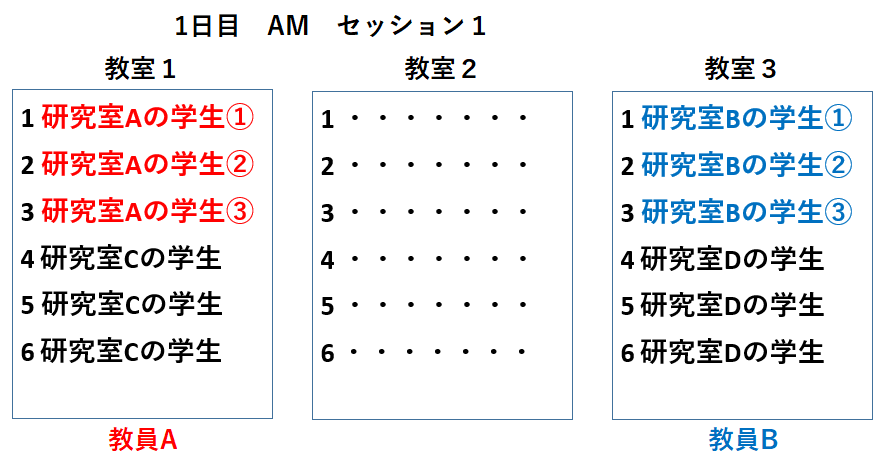
\includegraphics[width=10cm,height=4.5cm,]{BeforeOrder.PNG}
  \end{center}

 しかし、発表順序を考慮すると、図のように、研究室A と研究室B の学生の発表順序をずらすことが可能になります。よって、教員A は、自分の担当する学生の発表が終わり次第、教室を移動し、研究室B の学生の発表を聞きに行くことができます。

 \begin{center}
    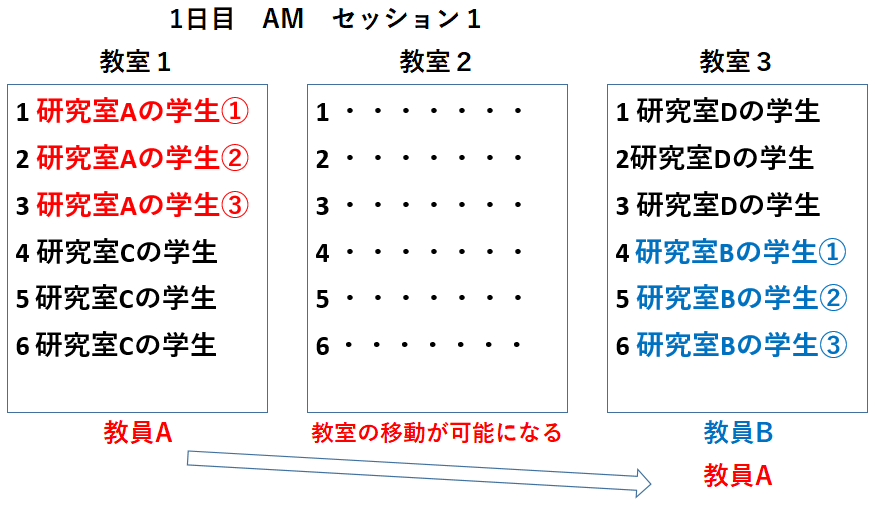
\includegraphics[width=10cm,height=4.5cm,]{AfterOrder.PNG}
  \end{center}

 以上が、現在頂いている要件の内容になります。\\
 
  
今回、より柔軟なスケジュールを作成するために、現在頂いている要件のような、スケジュール作成において追加・変更したい部分について、先生方からの意見を頂きたくこのアンケートを実施いたしました。スケジュール作成において、追加・変更したい部分があれば、お答えください。ご協力お願いします。



\end{document}
